\lecture{8}{21. April 2026}{Frequency Response Methods}

\section{Frequency Response Methods}

\subsection{Introduction and Concepts}
A frequency response describes how a system responds in steady-state when the input is sinusoidal.
So if the input is:
\begin{equation*}
  r(t) = A \sin \left( \omega t \right)
\end{equation*}
then, after the transient part has died away, the output of a linear time-invariant system will be sinusoidal.
The output here will have the \textit{same frequency}, but generally \textit{different amplitude and different phase}.
So the system does not change the frequency of the sinusoidal signal.
It only scales it and shifts it in time.

For example, if you input a slow sine wave into a mechanical system, the output may follow it almost perfectly.
If you input a very fast sine wave, the output may be much smaller and delayed.
This is exactly this dependency on frequency that frequency response studies.

In general, for a sinusoidal input
\begin{equation*}
  r(t) = A \sin (\omega t)
\end{equation*}
the output is
\begin{equation*}
  y(t) = \left| T(j\omega) \right|A \sin (\omega t + \theta)
.\end{equation*}
Where $\left| T(j\omega) \right|$ is the gain of the system at frequency $\omega$, which tells hoe much the amplitude is magnified, and $\theta = j \omega$ is the phase angle, which tells how much the output is shifted relative to the input.
Normally $\theta < 0$ in physical systems, meaning they lag behind as they cannot react instantly.

\subsubsection{Laplace vs. Fourier transform}
We have previously mainly been using Laplace transforms, defined as:
\begin{equation*}
  F(s) = \mathcal{L}\left\{ f(s) \right\} = \int_{0}^{\infty} f(t) e^{-st} \, \mathrm{d}t 
.\end{equation*}
Now, we introduce the Fourier transform, defined by:
\begin{equation*}
  F(\omega) = \mathcal{F}\left\{ f(t) \right\} = \int_{-\infty}^{\infty} f(t) e^{-j\omega t} \, \mathrm{d}t 
.\end{equation*}
The key difference between these is the complex variable.
For Laplace $s = \sigma + j\omega$, while for Fourier, we only use the imaginary axis $s = j\omega$.
So, the Fourier transform can be viewed as a special case of the Laplace transform, where we evaluate along the imaginary axis.
This is the reason frequency response uses $s = j\omega$, i.e. we are asking, ``what does the transfer function look like for pure sinusoidal motion at frequency $\omega$?''.
This happens as sinusoids are associated with complex exponentials, $e^{j\omega t}$, and therefore with the imaginary axis in the $s$-plane.
The inverse Fourier transform is given as:
\begin{equation*}
  y(t) = \frac{1}{2\pi} \int_{-\infty}^{\infty} Y(j\omega) e^{j\omega t} \, \mathrm{d}\omega
.\end{equation*}
This integral is usually difficult to compute directly, so instead of reconstructing $y(t)$ exactly, graphical and experimental methods are often used -- This is where Bode plots, and polar plots come in.
These lets us study the magnitude and phase of $T(j\omega)$ without needing to solve the full time-domain response every time.

In earlier control theory, the Laplace transform lets us study the pole-zero structure of $T(s)$, meaning we can study stability, transient behavior, damping, natural frequency, and so on.
But in frequency response methods, we evaluate the transfer function at $s = j\omega$, so we get $T(j\omega)$, which is now a frequency dependant complex number.
In the frequency domain, the transfer function $T(j\omega)$ is defined similarly as for the time domain
\begin{equation*}
  Y(j\omega) = T(j\omega)R(j\omega)
.\end{equation*}
For a closed-loop system this becomes:
\begin{equation*}
  T(j\omega) = \frac{G(j\omega)}{1 + G(j\omega) H(j\omega)}
.\end{equation*}
Which is just the usual closed-loop transfer function, but with $s$ replaced by $j\omega$.

\subsubsection{Advantages and Disadvantages of Frequency Response Methods}
Frequency response methods are useful in variety of ways.
Often, the frequency response can be obtained directly by testing the real system.
For example, you can apply sinusoidal inputs at different frequencies:
\begin{equation*}
  r(t) = A \sin (\omega t)
\end{equation*}
then measure the output amplitude and phase, from where $\left| T(j\omega) \right|$ and $j\omega$ can then be estimated. 

The second advantage is analytical.
If you already know the transfer function $T(s)$, you can get the frequency response by simply replacing $s$ with $j\omega$, so $T(s) \to T(j\omega)$, then you study how the complex number $T(j\omega)$ changes as $\omega$ increases.

The third advantage is graphical.
Magnitude and phase can be represented clearly using e.g. Bode plots, which show magnitude and phase versus frequency.

The disadvantages are also important.
Frequency response is not a time-domain method, so it does not show the exact time response to e.g. a step input at each frequency.
So in this way there is an indirect link between frequency domain information and time domain behavior.
For example, bandwidth, phase margin, gain margin, and resonance tell us a lot about speed, overshoot and stability, but the connection is not always as visually immediate as looking at a step response. 

\subsection{Polar Plots} \label{sec:polplot}
Once we replace $s$ by $j\omega$, the transfer function becomes a complex-valued function of frequency, so instead of writing only $G(s)$, we now write $G(j\omega)$, and because it is complex, it can be split into a real and an imaginary part
\begin{equation*}
  G(j\omega) = R(\omega) + j X(\omega)
.\end{equation*}
So, for every frequency $\omega$, the tranfer function gives one complex number.
That complex number can be drawn as a point in the complex plane on \Cref{fig:complex}.

The horizontal axis of \Cref{fig:complex} is the real part, $R(\omega)$ and the vertical axis is the imaginary part $X(\omega)$.

\begin{figure} [ht]
  \centering
  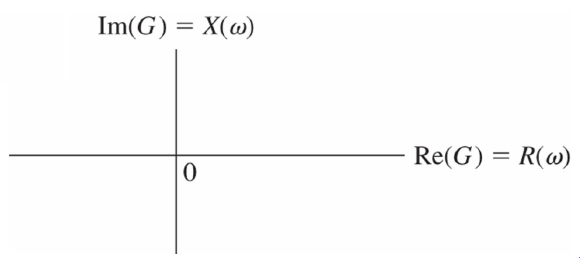
\includegraphics[width=0.8\linewidth]{./figures/complex.png}
  \caption{The complex plane}
  \label{fig:complex}
\end{figure}

The same complex number can also be written in polar form:
\begin{equation*}
  G (j\omega) = \left| G(j\omega) \right| e^{j\phi(\omega)}
\end{equation*}
or
\begin{equation*}
  G(j\omega) = \left| G(j\omega) \right| \angle \phi(\omega)
.\end{equation*}
The magnitude is:
\begin{equation*}
  \left| G(j\omega) \right| = \sqrt{R(\omega)^2 + X(\omega)^2}
\end{equation*}
and the phase is:
\begin{equation*}
  \phi(\omega) = \tan^{-1} \left( \frac{X(\omega)}{R(\omega)} \right)
.\end{equation*}
So the polar plot is simply the path traced by $G(j\omega)$ in the complex plane as $\omega$ changes.

\subsubsection{Example of Polar Plotting} \label{sec:RC}
We will now show this for a concrete example: an RC filter, shown on \Cref{fig:e8_1}.
The circuit has a resistor $R$ in the series and a capacitor $C$ to ground.
The input voltage is $V_1(s)$, and the output voltage $V_2(s)$ is measured across the capacitor.
This is a standard first-order low-pass filter.

\begin{figure} [ht]
  \centering
  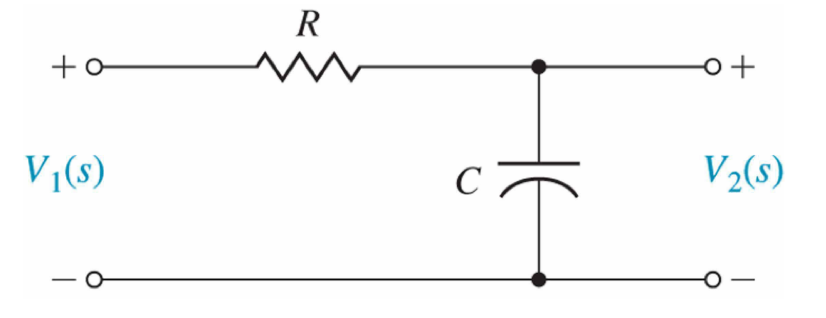
\includegraphics[width=0.6\linewidth]{./figures/e8_1.png}
  \caption{RC filter for example of polar plotting.}
  \label{fig:e8_1}
\end{figure}

At low frequency, the capacitor behaves almost like an open circuit.
So almost no current flows, meaning almost no voltage is lost across the resistor.
Therefore $V_2\approx V_1$.
At high frequency, the capacitor behaves almost like a short circuit to ground.
So the output node is pulled close to ground, meaning $V_2 \approx 0$.
So physically, we would expect this circuit to pass low frequencies and attenuate high frequencies.

To draw the pole plot, we must first derive the frequency domain transfer function of the system.
The circuit is just a voltage divider
\begin{equation*}
  G(s) = \frac{V_2(s)}{V_1(s)} = \frac{Z_C}{R + Z_C}
.\end{equation*}
Substituting the impedance of a capacitor, $Z_C = 1 /(sC)$, we obtain
\begin{equation*}
  G(s) = \frac{\frac{1}{sC}}{R + \frac{1}{SC}} = \frac{1}{RCs + 1}
.\end{equation*}
Now, we move into frequency response by replacing $s = j\omega$, so:
\begin{equation*}
  G(j\omega) = \frac{1}{j\omega RC + 1}
.\end{equation*}
Multiplying with the complex conjugate we obtain:
\begin{equation*}
  G(j\omega) = \frac{1-j\omega RC}{1 + \left( \omega RC \right)^2} = \frac{1}{1 + \left( \omega RC \right)^2} - j \frac{\omega RC}{1 + \left( \omega RC \right)^2}
.\end{equation*}
So, now we can identify:
\begin{equation*}
  R(\omega) = \frac{1}{1 + \left( \omega RC \right)^2}
\end{equation*}
and
\begin{equation*}
  X(\omega) = - \frac{\omega RC}{1 + \left( \omega RC \right)^2}
.\end{equation*}
We also define the corner frequency:
\begin{equation*}
  \omega_1 = \frac{1}{RC}
\end{equation*}
so that
\begin{equation*}
  \omega RC = \frac{\omega}{\omega_1}
.\end{equation*}
Which makes the equations cleaner:
\begin{equation*}
  G(j\omega) = \frac{1}{1 + \left( \frac{\omega}{\omega_1} \right)^2} - j \frac{\frac{\omega}{\omega_1}}{1 + \left( \frac{\omega}{\omega_1} \right)^2}
.\end{equation*}
The magnitude is
\begin{equation*}
  \left| G(j\omega) \right| = \frac{1}{\sqrt{1 + \left( \frac{\omega}{\omega_1} \right)^2}}
\end{equation*}
and the phase is:
\begin{equation*}
  \phi(\omega) = - \tan^{-1} \left( \frac{\omega}{\omega_1} \right)
.\end{equation*}

We can now turn the real and imaginary parts into a polar plot.
We have:
\begin{equation*}
  R(\omega) = \frac{1}{1 + \left( \frac{\omega}{\omega_1} \right)^2} \qquad X(\omega) = - \frac{\frac{\omega}{\omega_1}}{1 + \left( \frac{\omega}{\omega_1} \right)^2}
.\end{equation*}
Now, we look at a few important frequencies.
At $\omega = 0$, we get $R(0) = 1$, and $X(0) = 0$, so $G(j0) = 1$.
As the polar plot is in the complex plane (the $R$-$X$-plane in this context), it starts at the point $(1,0)$.
Physically, this means DC passes through the low-pass filter unchanged.

At $\omega = \omega_1$ we get $R(\omega_1) = 1 / 2$ and $X(\omega_1) = - 1 / 2$.
So the point corresponding to $\omega = \omega_1$ is $(1 / 2, - 1 / 2)$-
The magnitude is:
\begin{equation*}
  \left| G(j\omega_1) \right| = \sqrt{\left( \frac{1}{2} \right)^2 + \left( -\frac{1}{2} \right)^2} = \frac{1}{\sqrt{2}}
\end{equation*}
and the phase is:
\begin{equation*}
  \phi(\omega_1) = - \ang{45} 
.\end{equation*}
This is the familiar cutoff point of a first-order RC low-pass filter.

At $\omega \to \infty$, we get $R(\omega) \to \infty$ and $X(\omega) \to \infty$, so the plot approaches the origin.
Physically, very high-frequency signals are blocked.

For positive frequencies, the curve goes through the lower half of the complex plane because the imaginary part is negative, for negative frequencies, the curve mirrors the upper half-plane.
This is all shown on \Cref{fig:e8_11}.

\begin{figure} [ht]
  \centering
  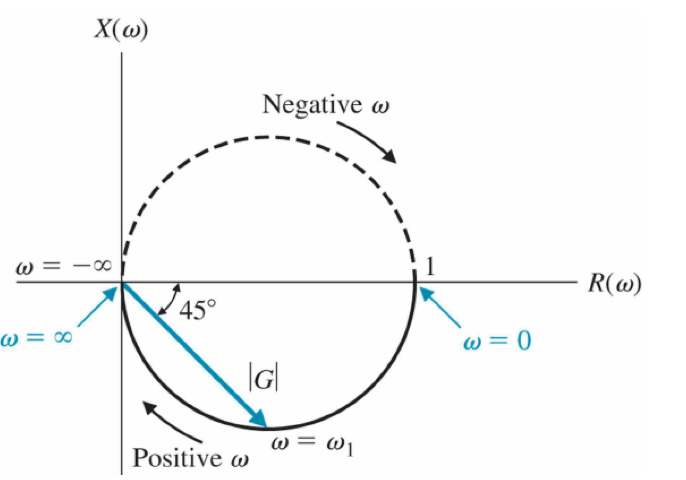
\includegraphics[width=0.5\linewidth]{./figures/e8_11.png}
  \caption{Polar plot of the RC filter}
  \label{fig:e8_11}
\end{figure}

Here, we see that the locus is a circle with centre $(1 / 2, 0)$ and radius $1 / 2$.
We see this by:
\begin{equation*}
  \left( R - \frac{1}{2} \right)^2 + X^2 =\left( \frac{1}{2}\right)^2
.\end{equation*}
So the RC filter's polar plot is a circle passing through $(1,0)$ and $(0,0)$ with its center at $(1 / 2, 0)$.

\subsubsection{The Limitations of Polar Plots}
Polar plots are useful because they show the complex value of $G(j\omega)$ directly.
They show both magnitude and phase in one curve, but they have limitations.
The first problem is that if you add another pole or zero to the system, the whole polar plot changes.

The second problem is that polar plots do not clearly show the individual effect of each pole and zero.
A pole contributes magnitude reduction and phase lag.
A zero contributed magnitude increase and phase lead.
But in a polar plot, these effects are mixed together in one curve.

\subsection{Bode Plots}
An alternative to polar plots introduced in \Cref{sec:polplot} are Bode plots.
For polar plots, we represented the frequency response as a complex number
\begin{equation*}
  G(j\omega) = \left| G(j\omega) \right|e^{j\phi(\omega)}
.\end{equation*}
So $G(j\omega)$ contains both information about magnitude ($\left| \ldots  \right|$) and phase angle ($\phi(\omega)$).
A Bode plot separates these into two plots: a magnitude plot in decibels versus frequency and a phase plot which shows the phase angle in degrees versus frequency.
The magnitude is not usually plotted directly as $\left| G(j\omega) \right|$.
Instead, it is plotted in decibels:
\begin{equation*}
  20 \log_{10} \left| G(j\omega) \right|
\end{equation*}
also known as the logarithmic gain.

The reason for using decibels is that multiplication becomes addition.
This is very useful when transfer functions contain many factors, e.g. if
\begin{equation*}
  G(j\omega) = G_1(j\omega) G_2(j\omega)
\end{equation*}
then
\begin{equation*}
  20 \log_{10} \left| G(j\omega) \right| = 20 \log_{10} \left| G_1 (j\omega) \right| + 20 \log_{10} \left| G_2 (j\omega) \right|
.\end{equation*}
So complicated transfer functions become much easier to sketch.

\subsubsection{Example of Bode Plotting}
Now, we move to the same RC low-pass filter as in \Cref{sec:RC}.
The transfer function was:
\begin{equation*}
  G(j\omega) = \frac{1}{j\omega RC + 1}
.\end{equation*}
We now define the time constant $\tau = RC$, so the transfer function may be written as
\begin{equation*}
  G(j\omega) = \frac{1}{j\omega t + 1}
.\end{equation*}
The magnitude is:
\begin{equation*}
  \left| G(j\omega) \right| = \frac{1}{\sqrt{1 + \left( \omega \tau \right)^2}}
.\end{equation*}
So the logarithmic gain is:
\begin{equation*}
  20 \log \left| G(j\omega) \right| = 20 \log \left( \frac{1}{\sqrt{1 + \left( \omega \tau \right)^2}} \right) = - 10 \log \left( 1 + \left( \omega \tau \right)^2 \right)
.\end{equation*}
The phase angle is then:
\begin{equation*}
  \phi(\omega) = - \tan^{-1} (\omega\tau)
.\end{equation*}
So the RC filter has magnitude decreasing with frequency, and phase becoming more negative with frequency.
This is shown on \Cref{fig:RCbode}.

\begin{figure} [ht]
  \centering
  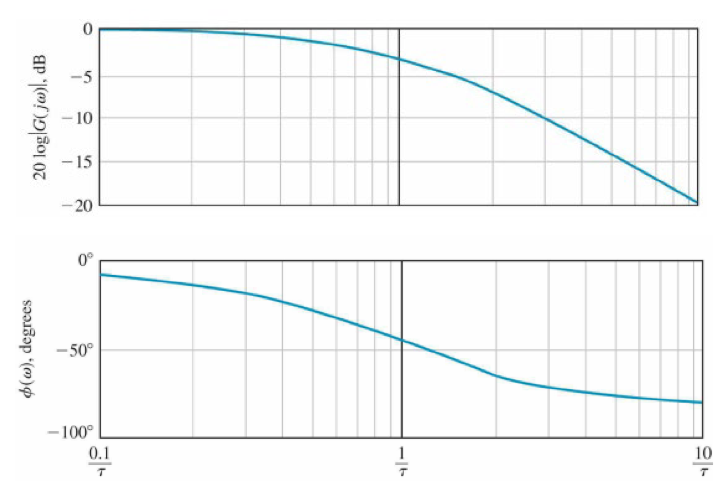
\includegraphics[width=0.5\linewidth]{./figures/RCbode.png}
  \caption{Bode plot of the RC-filter}
  \label{fig:RCbode}
\end{figure}

We not analyze the magnitude expression in three important regions.
When $\omega \ll 1 / \tau$, then $\omega \tau \ll 1$, so $1 + \left( \omega \tau \right)^2 \approx 1$, therefore, for $\omega \ll 1$:
\begin{equation*}
  20 \log \left| G(j\omega) \right| \approx -10 \log (1) = \qty{0}{\dB} 
.\end{equation*}
I.e. the filter passes low frequencies almost unchanged.

When $\omega \gg 1 / \tau$, then $1 + \left( \omega \tau \right)^2 \approx \left( \omega \tau \right)^2$, so 
\begin{equation*}
  20 \log \left| G(j\omega) \right| \approx - 10 \log \left( \left( \omega \tau \right)^2 \right) = - 20 \log \left( \omega \tau \right) 
.\end{equation*}
So after the corner frequency, the magnitude falls linearly on the logarithmic plot.

At the corner frequency, $\omega_c = 1 / \tau$, we get $\omega \tau = 1$, so $\left| G(j \omega_c) \right| = 1 / \sqrt{2}$.
In decibels this is:
\begin{equation*}
  20 \log \left( \frac{1}{\sqrt{2}} \right) = - \qty{3,01}{\dB} 
.\end{equation*}
Hence, why the corner frequency is also known as the \qty{-3}{\dB} frequency.
So for a first-order RC low-pass filter: $\omega_c = 1 / (RC)$ is the frequency where the amplitude has dropped to about \num{70,7} \% of the input amplitude.

\paragraph{Hand Sketching Bode Plots and Straight-Line Approximation}
Instead of drawing the exact curve, we can approximate it using straight-line asymptotes.
For the RC low-pass filter from before, at low frequency $\omega \ll 1 / \tau$, the magnitude is approximately \qty{0}{\dB}, so the first asymptote is a horizontal line.

At high frequencies, $\omega \gg 1 / \tau$, the magnitude is approximately $-20 \log (\omega \tau)$, which is a straight line with slope $-\qty{20}{\dB} / \text{decade}$, where a decade is a factor 10 in frequency.
I.e. going from $\omega$ to $10\omega$ is one decade.
This is shown on \Cref{fig:RCbodestraight}.

\begin{figure} [ht]
  \centering
  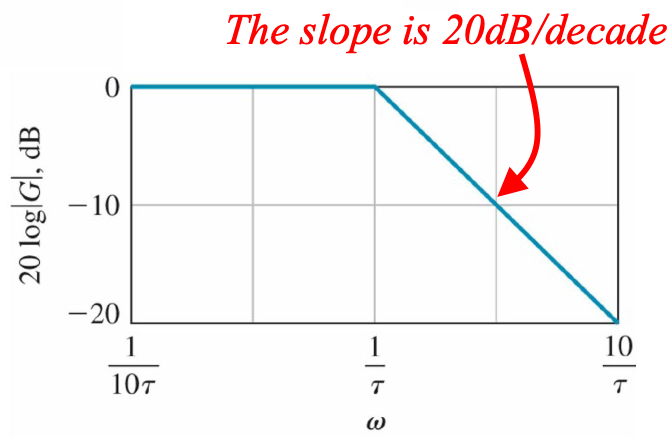
\includegraphics[width=0.5\linewidth]{./figures/RCbodestraight.png}
  \caption{Straight line approximation of the magnitude part of the bode plot on \Cref{fig:RCbode}.}
  \label{fig:RCbodestraight}
\end{figure}.

\paragraph{General Bode Plot Construction}
A general transfer function can be written as a product of simpler factors:
\begin{equation*}
  G(j\omega) = \frac{K_b \prod_{i = 1}^{Q} \left( 1 + j \omega\tau_i \right)}{\left( j\omega \right)^{N}\prod_{m = 1}^{M} \left( 1 + j \omega \tau_m \right) \prod_{k = 1}^{R} \left( 1 + 2 \frac{\xi_k}{\omega_{nk}} j \omega + \left( \frac{j \omega}{\omega_{nk}} \right)^2 \right)}
.\end{equation*}
This looks horrible, but the point is that it is built from simpler pieces.
There may be:
\begin{itemize}
  \item Constant gain $K_b$
  \item Zeros on the real axis
  \item Poles at the origin
  \item Poles on the real axis
  \item Complex conjugate pole pairs
\end{itemize}
The bode magnitude is bades on $20 \log \left| G(j\omega) \right|$.
Because of the logarithm, products become sums and divisions become subtractions.
So the total magnitude plot is:
\begin{equation*}
  \text{gain contributions} + \text{zero contributions} - \text{pole contributions}
.\end{equation*}
The same idea applies to the phase, where the total phase angle is the sum of the phase angles from each factor.
So instead of trying to plot the whole transfer function at once, Bode plots let us break it down factor by factor.

\subsubsection{The Four Basic Kinds of Factors}
Almost all transfer functions we meet in this course can be decomposed into four types of factors:
\begin{itemize}
  \item Constant gain, $K_b$.
    This just shifts the magnitude plot up or down.
  \item Poles or zeros at the origin.
    E.g. $j\omega$ or $1 / (j\omega)$.
    A zero at the origin behaves like a differentiator and a pole at the origin behaves like an integrator.
  \item Real-axis poles or zeros.
    E.g. $1 + j \omega\tau$ or $1 / (1 + j \omega \tau)$.
    These are first-order factors, exactly like the RC filter from the previous examples are.
  \item Complex conjugate poles or zeros.
    E.g.
    \begin{equation*}
      1 + 2 \xi \frac{j\omega}{\omega_n} + \left( \frac{j \omega}{\omega_n} \right)^2
    .\end{equation*}
    These are second-order factors and are important for systems with damping, resonance, overshoot, oscillation, and natural frequency.
\end{itemize}
The practical recipe is to first split the transfer function into the above factors.
Then find the magnitude and phase contributions from each factor.
Then, add all the magnitude together and add all the phase curves together.

\subsubsection{Bode Plot for Constant Gain}
This is the easiest factor, i.e. a constant gain.
If the transfer function is just:
\begin{equation*}
  G(j\omega) = K_b
\end{equation*}
then the magnitude is constant
\begin{equation*}
  20 \log \left| K_b \right|
.\end{equation*}
So on a Bode magnitude plot, this is a horizontal line.
E.g. $K_b = 10 \implies 20 \log (10) = \qty{20}{\dB}$ and $K_b = \num{0,1} \implies 20 \log (\num{0,1} ) = - \qty{20}{\dB}$.

If $K_b$ is positive, the phase angle is $\phi(\omega) = \ang{0}$, because multiplying by a positive number does not shift the signal in phase.
If the gain is negative, e.g.
\begin{equation*}
  G(j\omega) = - K_b
\end{equation*}
then, the magnitude is still:
\begin{equation*}
  20 \log \left| K_b \right|
\end{equation*}
but the phase is shifted by \ang{-180}.

\subsubsection{Poles and Zeros at the Origin}
Factors like
\begin{equation*}
  \left( j\omega \right)^{N}
\end{equation*}
and
\begin{equation*}
  \frac{1}{\left( j\omega \right)^{N}}
\end{equation*}
contribute zeros or poles at the origin because the corresponding factor is located at $s = 0$.

\paragraph{Pole at the origin}
For a pole at the origin:
\begin{equation*}
  G(j\omega) = \frac{1}{\left( j\omega \right)^{N}}
\end{equation*}
the magnitude is:
\begin{equation*}
  20 \log \left| \frac{1}{\left( j\omega \right)^{N}} \right| = - 20 N \log \omega
\end{equation*}
so the slope is $-20N \, \unit{\dB} / \text{decade}$.
I.e. for one pole at the origin the slope is $-\qty{20}{\dB} / \text{decade}$ whilst two poles at the origin gives a slope of $- \qty{40}{\dB}$.

The phase is:
\begin{equation*}
  \phi(\omega) = - \ang{90} N
.\end{equation*}
So one integrator gives \ang{-90}, and two integrators give \ang{-180}.

\paragraph{Zero at the Origin}
For a zero at the origin:
\begin{equation*}
  G(j\omega) = \left( j\omega \right)^{N}
.\end{equation*}
The magnitude is
\begin{equation*}
  20 \log \left| \left( j\omega \right)^{N} \right| = 20 N \log \omega
\end{equation*}
so the slope is $20 N \, \unit{\dB} / \text{decade}$.

The phase is:
\begin{equation*}
  \phi(\omega) = + \ang{90} N
.\end{equation*}
So poles at the origin makes the magnitude slope downward, while zeros at the origin make it slope upward.

The effects of poles and zeros at the origin are shown graphically on \Cref{fig:bodepolezero}.

\begin{figure} [ht]
  \centering
  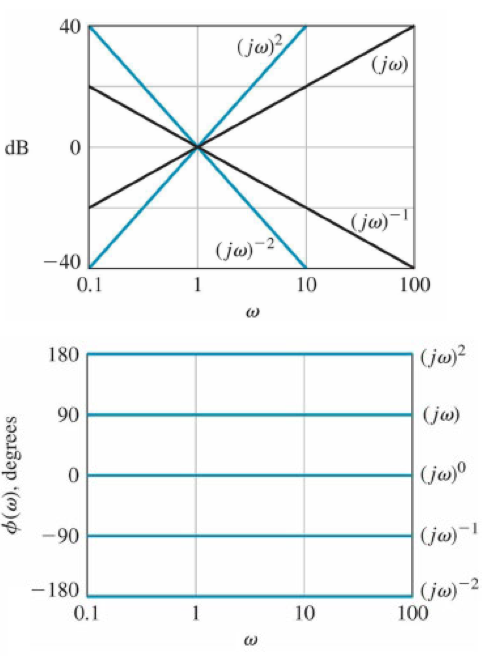
\includegraphics[width=0.4\linewidth]{./figures/bodepolezero.png}
  \caption{Effect of poles and zeros at the origin on Bode plots}
  \label{fig:bodepolezero}
\end{figure}

\subsubsection{Real-Axis Poles and Real-Axis Zeros}
For a first-order factor:
\begin{equation*}
  \frac{1}{1 + j\omega \tau}
\end{equation*}
we get a real-axis pole.

The magnitude of this is
\begin{equation*}
  20 \log \left| \frac{1}{1 + j\omega \tau} \right| = - 10 \log \left( 1 + \left( \omega \tau \right)^2 \right)
\end{equation*}
and the phase is
\begin{equation*}
  \phi(\omega) = - \tan^{-1}(\omega\tau)
.\end{equation*}

The corner frequency is $\omega_c = 1 / \tau$.
For frequencies much smaller than the corner frequency $\omega \ll  1 / \tau$, we have $1 + j\omega \tau \approx 1$, so the magnitude is approximately \qty{0}{\dB}.
For frequencies much larger than the corner frequency, $\omega \gg 1 / \tau$, the magnitude falls with slope $-\qty{20}{\dB} / \text{decade}$.
So the asymptotic approximation is flat before the corner frequency and then slopes downward after it.

The phase goes from $\ang{0} \to \ang{90} $, with the midpoint at the corner frequency, where $\phi = \ang{-45}$.

For a zero:
\begin{equation*}
  1 + j\omega \tau
\end{equation*}
the magnitude after the corner frequency is $+\qty{20}{\dB} / \text{decade}$, and the phase goes from $\ang{0}  \to \ang{90} $.
So the rule is a real pole bends the magnitude downward and adds phase lag, whilst a real zero bends the magnitude upward and adds phase lead.
This is all summarized graphically for a pole on the real axis on \Cref{fig:boderealpole}.

\begin{figure} [ht]
  \centering
  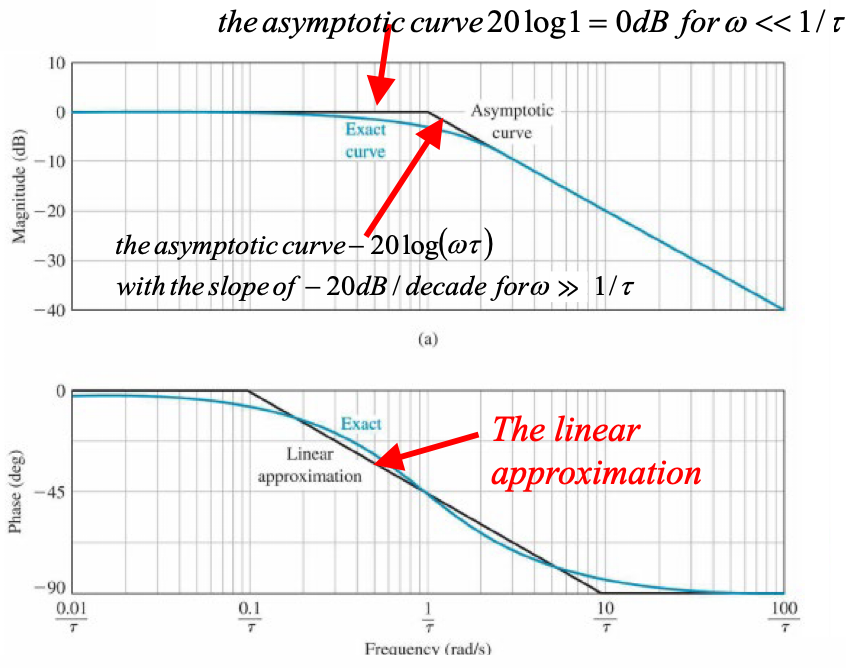
\includegraphics[width=0.5\linewidth]{./figures/boderealpole.png}
  \caption{Graphical representation of the effect of a pole on the real axis on a Bode plot.}
  \label{fig:boderealpole}
\end{figure}

\subsubsection{Complex Conjugate Poles or Zeros}
Now, we move to second-order factors.
A standard second-order pole pair has the form:
\begin{equation*}
  G(j\omega) = \frac{1}{1 + 2 \xi \frac{j\omega}{\omega_n} + \left( \frac{j\omega}{\omega_n} \right)^2}
.\end{equation*}
We now introduce the frequency ratio:
\begin{equation*}
  u = \frac{\omega}{\omega_n}
.\end{equation*}
Then the magnitude becomes:
\begin{equation*}
  20 \log \left| G(j\omega) \right| = -10 \log \left( \left( 1 - u^2 \right)^2 + 4 \xi^2 u^2 \right)
.\end{equation*}
And the phase becomes:
\begin{equation*}
  \phi(\omega) = - \tan^{-1} \left( \frac{2 \xi u}{1 - u^2} \right)
.\end{equation*}

The important new feature for this case is resonance.
For low damping, the magnitude can rise above \qty{0}{\dB} near the natural frequency.
This peak is called the resonant peak.
The resonant frequency is:
\begin{equation*}
  \omega_r = \omega_n \sqrt{1 - 2 \xi^2}
.\end{equation*}
This only exists as a real resonant \textit{peak} when the damping is sufficiently small.
The maximum magnitude at this peak is:
\begin{equation*}
  M_{p\omega} = \left| G(j\omega_r) \right| = \left( 2 \xi \sqrt{1 - \xi^2} \right)^{-1}
.\end{equation*}
So when $\xi$ is small (a lightly damped system) the resonant peak becomes large.
The magnitude plot on \Cref{fig:bodeconj} shows this clearly.
For small damping ratios, the curve has a tall peak near $\omega_n$, whilst for larger ratios, the peak becomes smaller or even disappears.

\begin{figure} [ht]
  \centering
  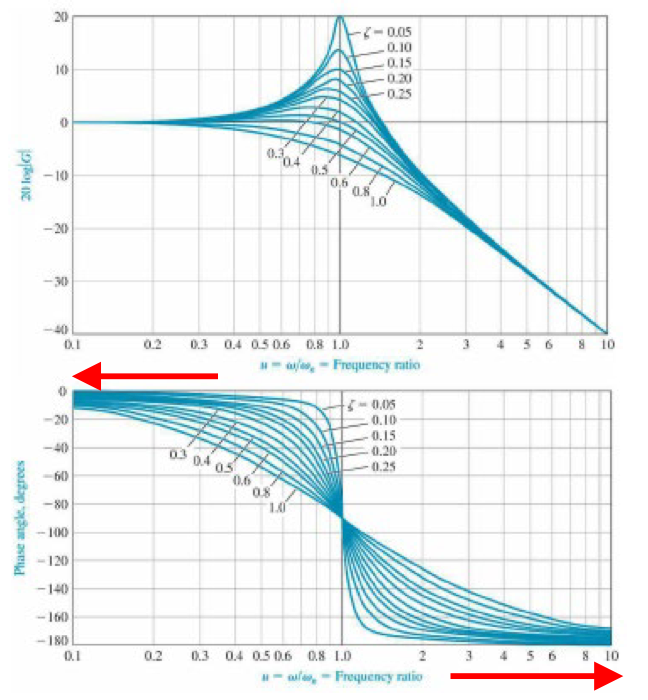
\includegraphics[width=0.5\linewidth]{./figures/bodeconj.png}
  \caption{Graphical representation of the effect of complex conjugate poles on the Bode plots.}
  \label{fig:bodeconj}
\end{figure}

The phase plot on \Cref{fig:bodeconj} shows that a second-order pole pair changes phase from $\ang{0} \to \ang{-180}$, with the transition being sharper for smaller damping.
So compared with a first-order pole, a second-order pole pair contributed twice as much final phase lag and twice the high-frequency magnitude slope: $-\qty{40}{\dB} / \text{decave}$. 

\begin{figure} [ht]
  \centering
  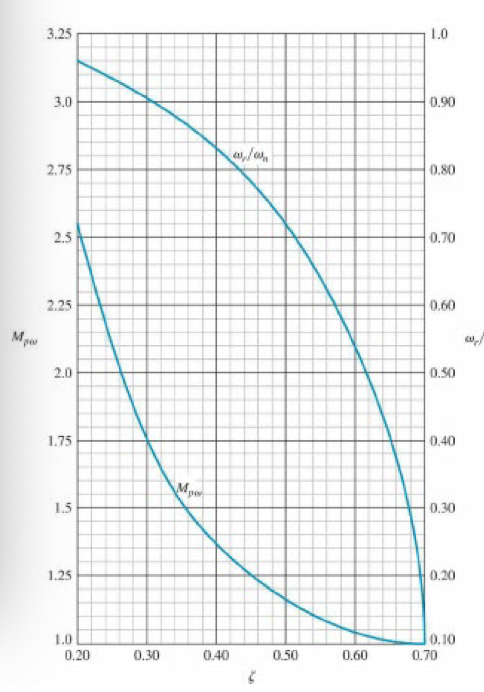
\includegraphics[width=0.25\linewidth]{./figures/xieffect.png}
  \caption{Effect of varying $\xi$ on the resonant frequency and the resonant peak.}
  \label{fig:xieffect}
\end{figure}

Second-order frequency response is very useful experimentally.
As the resonant peak and resonant frequency depend on the damping ratio $\xi$, if you can experimentally test a system and obtain its frequency response you can also estimate the damping ratio.
For example, if the Bode magnitude plot has a large resonant peak, the system is lightly damped, and if the peak is small the system is more heavily damped.
The graph on \Cref{fig:xieffect} shows how varying the damping ratio changes the resonant peak and resonant frequency.

All of the above results are also shown in \Cref{fig:asympcurve}.

\begin{figure} [ht]
  \centering
  \begin{subfigure}[t]{\textwidth}
    \centering
    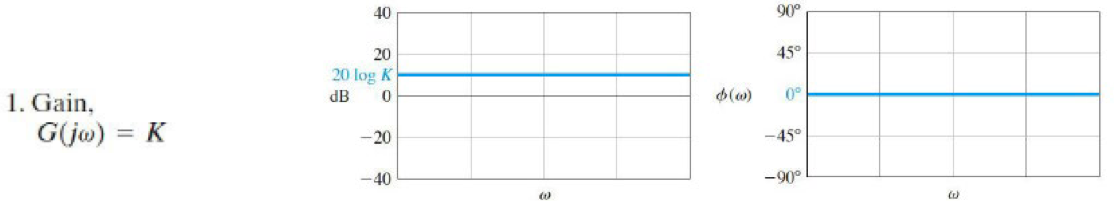
\includegraphics[height=0.8in]{./figures/asympcurve1.png}
    \caption{Asymptotic curve for the gain term of a transfer function.}
  \end{subfigure}
  \\
  \begin{subfigure}[t]{\textwidth}
    \centering
    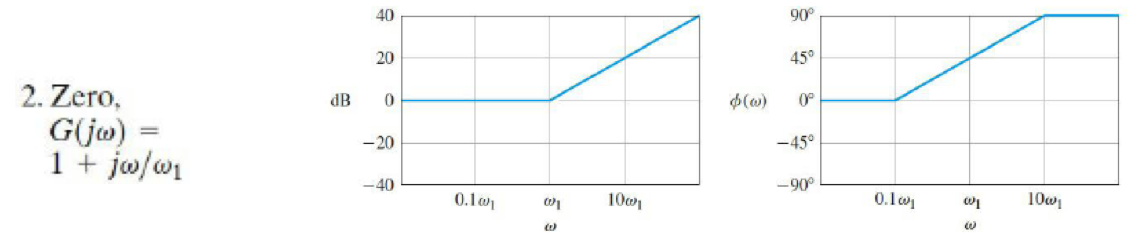
\includegraphics[height=0.9in]{./figures/asympcurve2.png}
    \caption{Asymptotic curve for a zero term of a transfer function.}
  \end{subfigure}
  \\
  \begin{subfigure}[t]{\textwidth}
    \centering
    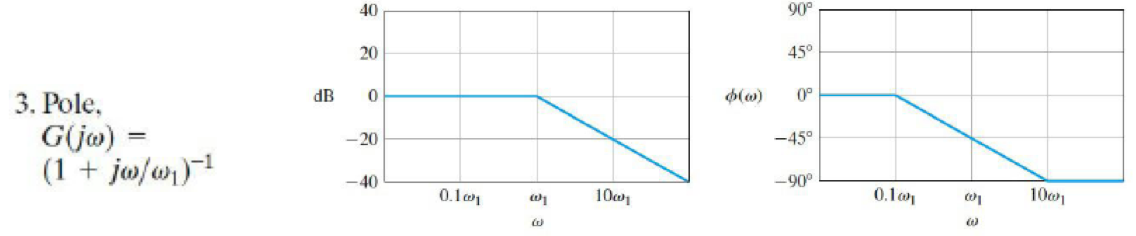
\includegraphics[height=0.92in]{./figures/asympcurve3.png}
    \caption{Asymptotic curve for a pole term of a transfer function.}
  \end{subfigure}
  \\
  \begin{subfigure}[t]{\textwidth}
    \centering
    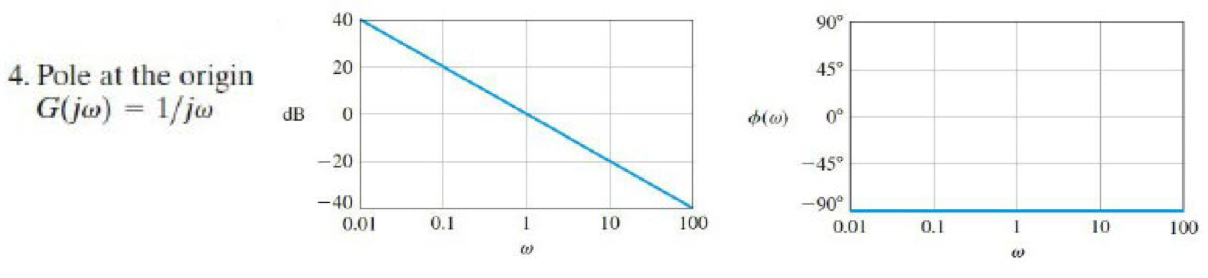
\includegraphics[height=1in]{./figures/asympcurve4.png}
    \caption{Asymptotic curve for a pole at the origin term of a transfer function.}
  \end{subfigure}
  \\
  \begin{subfigure}[t]{\textwidth}
    \centering
    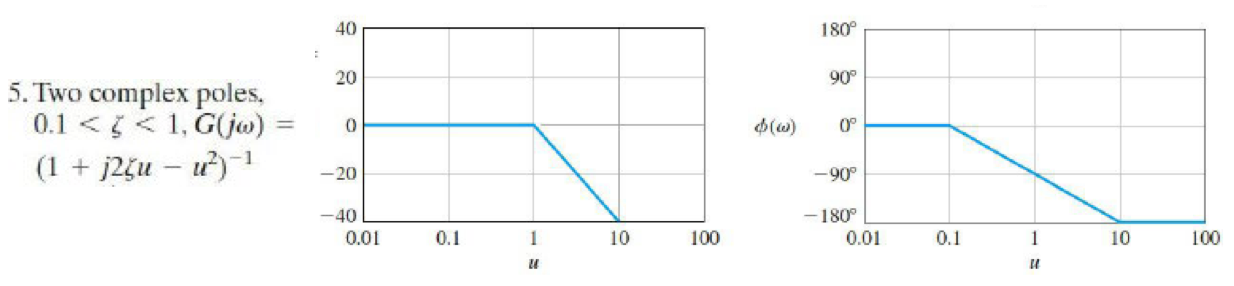
\includegraphics[height=1in]{./figures/asympcurve5.png}
    \caption{Asymptotic curve for two complex conjugate pole term of a transfer function.}
  \end{subfigure}
  \caption{Asymptotic curves for basic terms of a transfer function.}
  \label{fig:asympcurve}
\end{figure}

\subsubsection{Bode Plots in MatLab}
Creating a Bode plot in MatLab is easy, you simply use the \verb"bode" command.
E.g. for a system with transfer function:
\begin{equation*}
  G(j\omega) = \frac{5(1 + j \num{0,1} \omega)}{j\omega (1 + j \num{0,5} \omega) \left( 1 + j \num{0,6}  \left( \frac{\omega}{50} \right) + \left( \frac{j\omega}{50} \right)^2 \right)}
.\end{equation*}
We can sketch the Bode plots using the following code:
\begin{verbatim}
  num=5*[0.1 1];
  f1=[1 0];
  f2=[0.5 1];
  f3=[1/2500 .6/50 1];
  den=conv(f1, conv(f2, f3));
  sys=tf(num,den)
  bode(sys)
\end{verbatim}
Which yields the plot on \Cref{fig:matlabbode}.

\begin{figure} [ht]
  \centering
  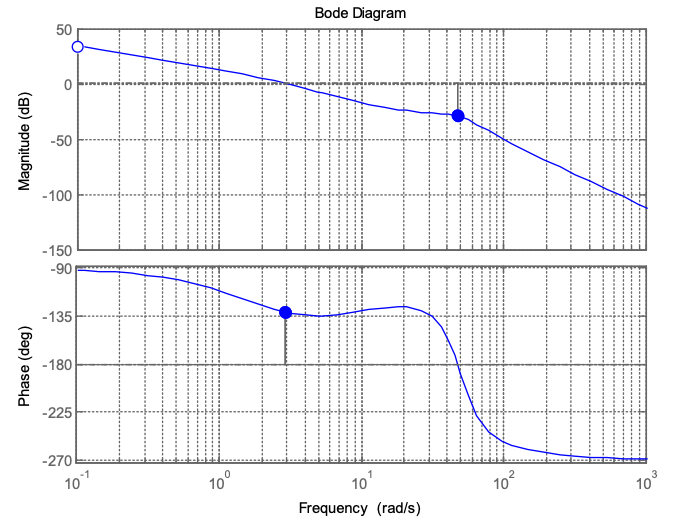
\includegraphics[width=0.4\linewidth]{./figures/matlabbode.png}
  \caption{Example Bode plot produced in MatLab.}
  \label{fig:matlabbode}
\end{figure}

\subsubsection{Basic Steps for Sketching Bode Plots}

\paragraph{Step 1: Rewrite in Proper Form}
We want each factor to look like on of the standard Bode factors:
\begin{gather*}
  K \\
  j\omega \\
  1 + \frac{j\omega}{\omega_1} \\
  \left( 1 + \frac{j\omega}{\omega_1} \right)^{-1} \\
  1 + 2 \xi \frac{s}{\omega_n} + \left( \frac{s}{\omega_n} \right)^2
.\end{gather*}
To do this we first want to make the lowest-order term unity.
For example,
\begin{equation*}
  s + 10
\end{equation*}
should be rewritten as
\begin{equation*}
  10 \left( 1 + \frac{s}{10} \right)
\end{equation*}
because now the term inside the brackets has constant term 1, and the break frequency is visible.
Similarly,
\begin{equation*}
  s + 3
\end{equation*}
should be rewritten as
\begin{equation*}
  3 \left( 1 + \frac{s}{3} \right)
.\end{equation*}
This is important as Bode sketching depends on seeing break frequencies directly.

\paragraph{Step 2: Replace $s$ by $j \omega$}
Once the transfer function is on the proper form per step 1, set
\begin{equation*}
  s = j \omega
\end{equation*}
because the Bode plot describes the steady-state response to sinusoidal inputs.

\paragraph{Step 3: Separate into constituent parts}
We now decompose the transfer function into:
\begin{itemize}
  \item constant gain
  \item zeros
  \item poles at the origin
  \item real poles
  \item complex poles
\end{itemize}
where each one has a known Bode contribution.

\paragraph{Step 4: Draw each part}
Now, the magnitude and phase contribution of each individual term is drawn.

\paragraph{Step 5: Add the results}
The final Bode plot is obtained by adding all magnitude curves in \unit{\dB} and adding all phase curves in degrees.

\begin{exa}[Example of Sketching a Bode Plot]
  Given the transfer function:
  \begin{equation*}
    G(s) = \frac{2500 (10 + s)}{s(s+2) \left( s^2 + 30s + 2500 \right)}
  .\end{equation*}
  We want to sketch the Bode plot of the system
  \tcblower
  The first step is to rewrite this so all factors have unity lowest-order term.
  First, we rewrite the numerator:
  \begin{equation*}
    10 + s = 10 \left( 1 + \frac{s}{10} \right)
  .\end{equation*}
  Now, we rewrite the first real pole:
  \begin{equation*}
    s + 2 = 2 \left( 1 + \frac{s}{2} \right)
  .\end{equation*}
  Then, we rewrite the second-order denominator:
  \begin{equation*}
    s^2 + 30s + 2500 = 2500 \left( 1 + \frac{30}{2500}s + \frac{s^2}{2500} \right) = 2500 \left( s + \num{0,6} \frac{s}{50} + \left( \frac{s}{50} \right)^2 \right)
  .\end{equation*}
  Now we collect the constants in the transfer function:
  \begin{equation*}
    G(s) = \frac{5  \left( 1 + \frac{s}{10} \right)}{s \left( 1 + \frac{s}{2} \right) \left( 1 + \num{0,6} \frac{s}{50} + \left( \frac{s}{50} \right)^2 \right)}
  .\end{equation*}
  
  Now, we replace $s$ with $j\omega$ leading to:
  \begin{equation*}
    G(j\omega) = \frac{5 \left( 1 + \frac{j\omega}{10} \right)}{j\omega \left( 1 + \frac{j\omega}{2} \right) \left( 1 + j \num{0,6} \frac{\omega}{50} + \left( \frac{j \omega}{50} \right)^2 \right)}
  .\end{equation*}
  This makes all the Bode factors visible.

  Now we determine the magnitude contribution of each part.
  From the transfer function we identify a constant gain $K = 5$.
  \begin{equation*}
    20 \log(5) \approx \qty{14}{\dB} 
  \end{equation*}
  so this contributes a horizontal line at \qty{14}{\dB}.

  We also have a pole at the origin:
  \begin{equation*}
    \frac{1}{/j\omega}
  .\end{equation*}
  This contributes \qty{-20}{\dB/dec} over the entire frequency range.
  It crosses \qty{0}{\dB} at $\omega = 1$ because
  \begin{equation*}
    20 \log \left( \frac{1}{1} \right) = 0
  .\end{equation*}
  
  We also have a real pole at $\omega = 2$ given by
  \begin{equation*}
    \frac{1}{1 + \frac{j\omega}{2}}
  .\end{equation*}
  This contributes \qty{0}{\dB} before $\omega = 2$ and \qty{-20}{\dB/dec} after $\omega = 2$

  The zero at $\omega = 10$ caused by
  \begin{equation*}
    1 + \frac{j\omega}{10}
  \end{equation*}
  contributes \qty{0}{\dB} before $\omega = 10$ and \qty{20}{\dB/dec} after $\omega = 10$.

  We also have a complex pole pair at $\omega = 50$ caused by:
  \begin{equation*}
    1 + j \num{0,6} \frac{\omega}{50} + \left( \frac{j\omega}{50} \right)^2
  .\end{equation*}
  This contributes \qty{0}{\dB} before $\omega = 50$ and \qty{-40}{\dB/dec} after $\omega = 50$.
  These individual contributions are shown on \Cref{fig:bodeconex}.

  We can now add  the magnitude curves.
  At low frequency, before $\omega = 2$, the only frequency dependent term is the pole at the origin.
  So the slope is \qty{-20}{\dB/dec}.
  At $\omega = 2$, the real pole begins to contribute another \qty{-20}{\dB/dec} leading the total slope to become \qty{-40}{\dB/dec}.
  At $\omega = 10$ the zero contributes \qty{20}{\dB/dec} so the slope changes to \qty{-20}{\dB/dec}.
  At $\omega = 50$, the complex pole pair contributes \qty{-40}{\dB/dec} so the final slope becomes \qty{-60}{\dB/dec}.
  This is shown on \Cref{fig:bodex}.

  Now we do the same thing for the phase.
  The constant gain $K = 5$ contributes \ang{0}.
  The pole at the origin $1 / (j\omega)$ gives \ang{-90} for all frequencies, so the phase starts at \ang{-90}.

  The real pole at $\omega = 2$ is a first order pole contributing from \ang{0} to \ang{-90}.
  This transition is sketched on \Cref{fig:bodeconexphase}, from $\num{0,1} \cdot 2 = \num{0,2} $ to $10 \cdot 2 = 20$.
  At the break frequency $\omega = 2$, the contribution is \ang{-45}.
  
  The zero at $\omega = 10$ is a first order zero contributing from \ang{0}  to \ang{90}.
  This is sketched from $\num{0,1} \cdot 10 = 1$ to $10 \cdot 10 = 100$.
  At $\omega = 10$, the contribution is \ang{45}. 

  The complex pole pair at $\omega = 50$ contributes from \ang{0} to \ang{-180}.
  The transition is from $\num{0,1} \cdot 50 = 5$ to $10 \cdot 50 = 500$, and at $\omega = 50$, the contribution is \ang{-90}.
  The final phase at very high frequency is therefore $\ang{-90} -\ang{90} +\ang{90} -\ang{180} =\ang{-270}$.
  This is shown on \Cref{fig:bodexphase}.

  The final Bode plot is the same as \Cref{fig:matlabbode}.
\end{exa}

\begin{figure} [ht]
  \centering
  \begin{subfigure}[t]{0.48\textwidth}
    \centering
    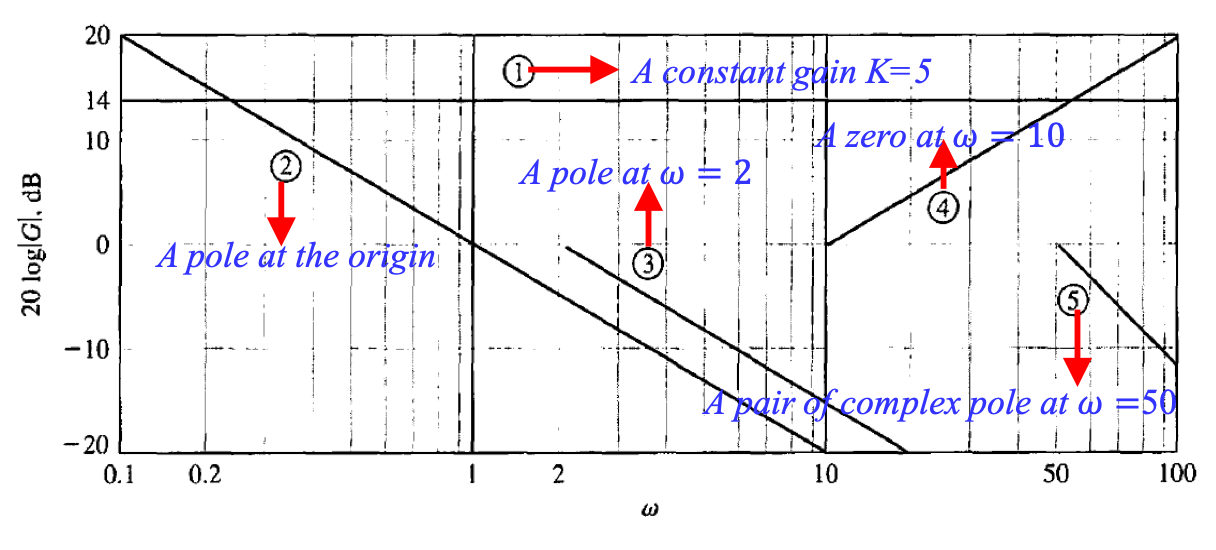
\includegraphics[width=\linewidth]{./figures/bodeconex.png}
    \caption{Contributions of the individual terms in the example Bode magnitude plot.}
    \label{fig:bodeconex}
  \end{subfigure}
  \hfill
  \begin{subfigure}[t]{0.48\textwidth}
    \centering
    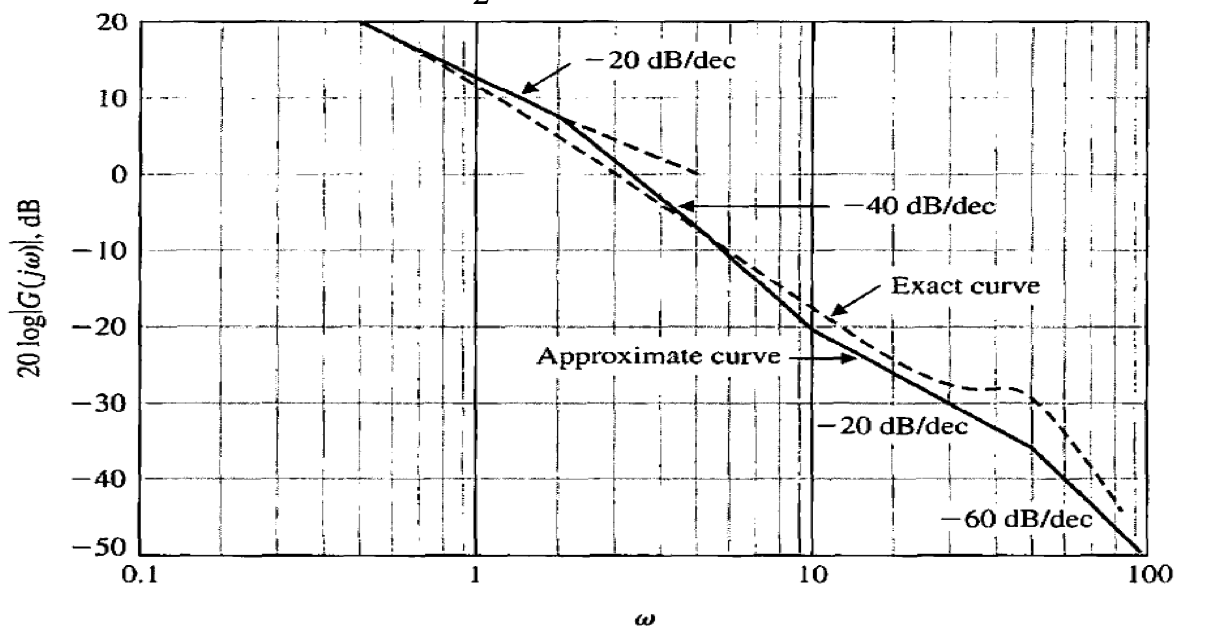
\includegraphics[width=\linewidth]{./figures/bodex.png}
    \caption{Bode magnitude plot of example system.}
    \label{fig:bodex}
  \end{subfigure}
  \\
  \begin{subfigure}[t]{0.48\textwidth}
    \centering
    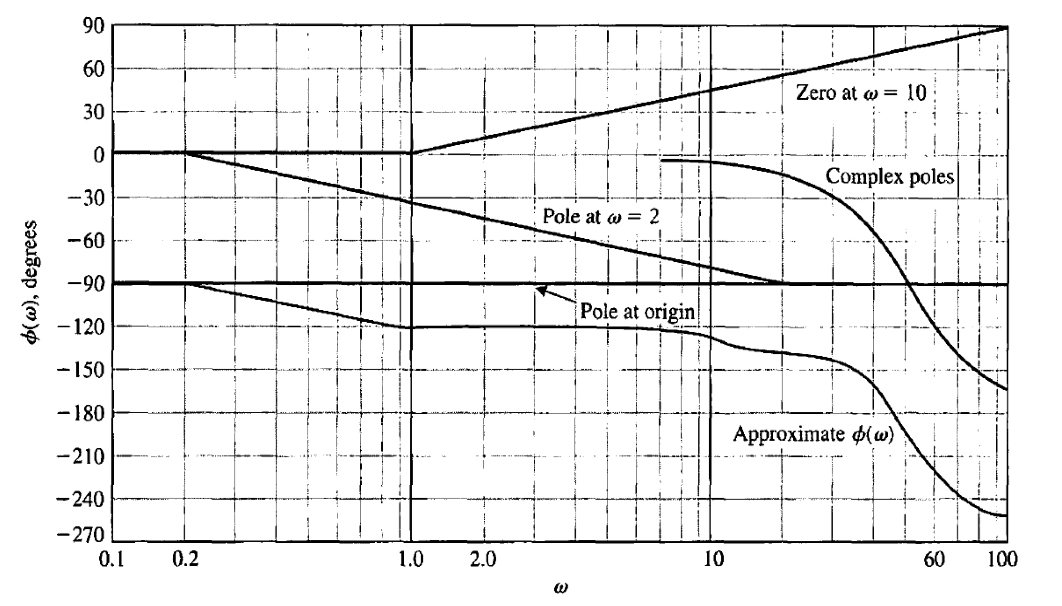
\includegraphics[width=\linewidth]{./figures/bodeconexphase.png}
    \caption{Contributions of the individual terms in the example Bode phase plot.}
    \label{fig:bodeconexphase}
  \end{subfigure}
  \hfill
  \begin{subfigure}[t]{0.48\textwidth}
    \centering
    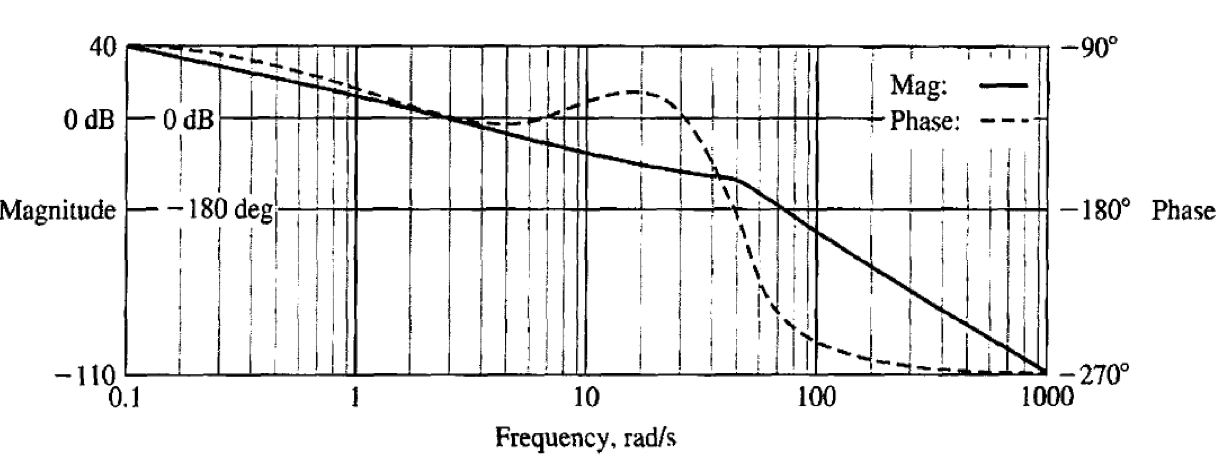
\includegraphics[width=\linewidth]{./figures/bodexphase.png}
    \caption{Bode phase plot of example system.}
    \label{fig:bodexphase}
  \end{subfigure}
\end{figure}

\subsection{Performance Specification}

\subsubsection{Bandwidth}
The bandwidth $\omega_B$ is defined as the frequency has dropped by \qty{3}{\dB} from its low-frequency value.
So if the low-frequency value is \qty{0}{\dB}, the bandwidth occurs at \qty{-3}{\dB}.
In ordinary magnitude, \qty{-3}{\dB} corresponds to
\begin{equation*}
  10^{-\frac{3}{20}}\approx \num{0,707} \approx \frac{1}{\sqrt{2}}
.\end{equation*}
So the bandwidth is the frequency, where the system output amplitude has fallen to about \num{70,7}\% of the low-frequency amplitude.
This often functions as a useful cutoff frequency.
Below $\omega_B$, the system reproduces inputs fairly well, whilst above $\omega_B$, the system attenuates systems more strongly.
I.e. the bandwidth of the closed-loop control system measures the range of frequencies over which the system can faithfully reproduce the input.

For example, suppose the reference signal contains both slow and fast components.
If the system has low bandwidth, it may follow the slow variations but fail to track the fast ones.
If the system has high bandwidth it can respond to faster variations.
So in this manner, bandwidth is a measure of tracking ability.
In general, a higher $\omega_B$ corresponds to faster step response and shorter settling time.

\begin{exa}[First-order Example: Larger Bandwidth Gives Faster Response]
  We compare the two first-order closed loop systems:
  \begin{align*}
    T_1(s) &= \frac{1}{s+1} \\
    T_2(s) &= \frac{1}{5s +1}
  .\end{align*}
  \tcblower
  We start by rewriting $T_2$ slightly as:
  \begin{equation*}
    T_2(s) = \frac{1}{5s +1} = \frac{\num{0,2} }{s + \num{0,2}}
  .\end{equation*}
  So $T_1$ has a pole at $s = -1$ and $T_2$ has a pole at $s = -\num{0,2}$.
  For a first-order system,
  \begin{equation*}
    T(s) = \frac{1}{\tau s + 1}
  \end{equation*}
  the bandwidth is approximately $\omega_B = 1 / \tau$.
  So for $T_1$,
  \begin{equation*}
    \tau_1 = 1 \implies \omega_B = 1
  \end{equation*}
  and for $T_2$,
  \begin{equation*}
    \tau_2 = 5 \implies \omega_B = \num{0,2} 
  .\end{equation*}
  So $T_1$ has a 5x larger bandwidth meaning $T_1$ is faster.
  This is also shown on the step input plot and ramp input plots on \Cref{fig:stepramp}.
\end{exa}

\begin{figure} [ht]
  \centering
  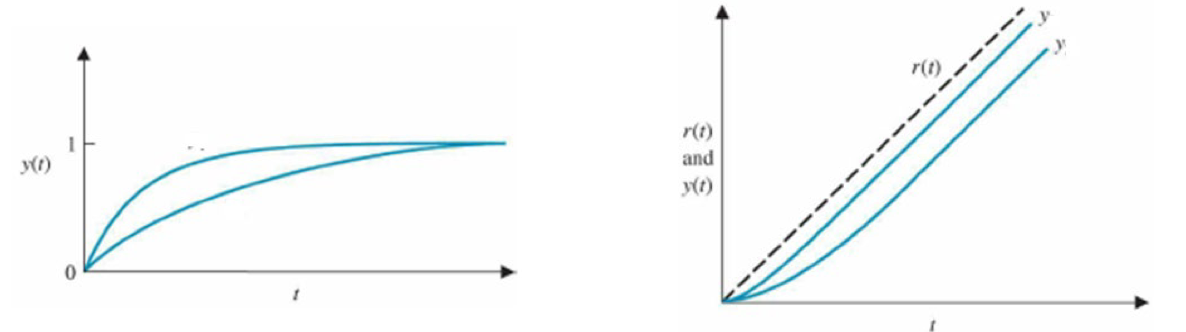
\includegraphics[width=0.8\linewidth]{./figures/stepramp.png}
  \caption{Step and ramp responses for the two first-order systems with different bandwidths.}
  \label{fig:stepramp}
\end{figure}

\begin{exa}[Second-Order Example: Same Damping; Different Natural Frequency]
  Now we are concerned with two second-order systems:
  \begin{align*}
    T_3(s) &= \frac{100}{s^2 + 10s + 100} \\
    T_4(s) &= \frac{900}{s^2 + 30s + 900}
  .\end{align*}
  \tcblower
  Comparing these with the standard second-order form:
  \begin{equation*}
    T(s) = \frac{\omega_n^2}{s^2 + 2\xi \omega_n s + \omega_n^2}
  .\end{equation*}
  For $T_3$, $\omega_n^2 = 100 \implies \omega_n = 10$ and $2 \xi \omega_n = 10 \implies \xi = \num{0,5}$.
  And for $T_4$, $\omega_n^2 = 900 \implies \omega_n = 30$ and $2\xi \omega_n = 30 \implies \xi = \num{0,5}$.
  So the two systems have the same damping ratio, but different natural frequencies. 

  Because $T_4$ has a natural frequency three times larger, it is basically a faster version of $T_3$.
  This is also evident on \Cref{fig:2ordex}, where the table shows that the bandwidth triples.
  The overshoot however stays the same as this depends mainly on the damping ratio $\xi$, which is equal for both systems.
  However both the peak time and settling time is approximately three times quicker for the system with the higher natural frequency.
\end{exa}

\begin{figure} [ht]
  \centering
  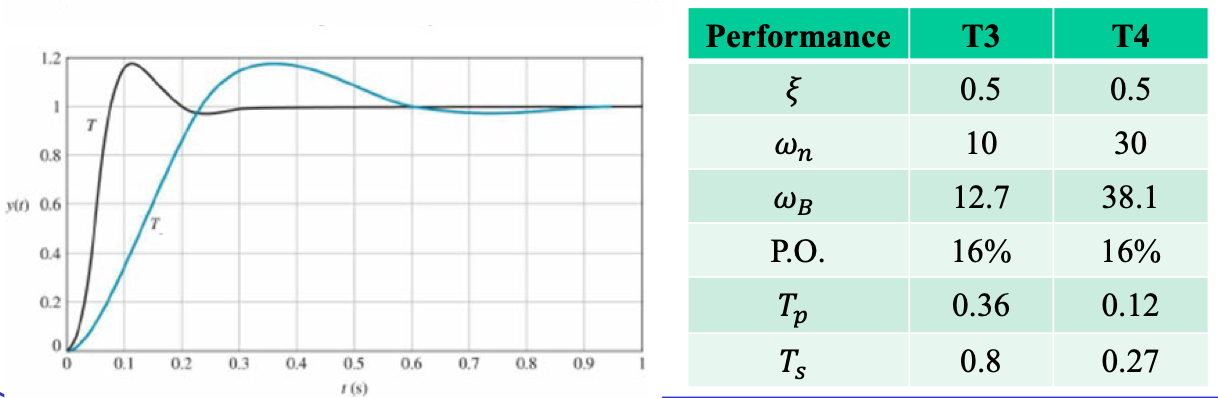
\includegraphics[width=0.8\linewidth]{./figures/2ordex.png}
  \caption{Comparison of the two second-order systems for a step input and for various important parameters.}
  \label{fig:2ordex}
\end{figure}

In general, the bandwidth $\omega_B$ of a second order system:
\begin{equation*}
  T(s) = \frac{\omega_n^2}{s^2 + 2\xi \omega_n s + \omega_n^2}
\end{equation*}
is related to the natural frequency $\omega_n$.
A plot of $\omega_B / \omega_n$ against damping ratio $\xi$ is shown on \Cref{fig:bandwidth}. 

\begin{figure} [ht]
  \centering
  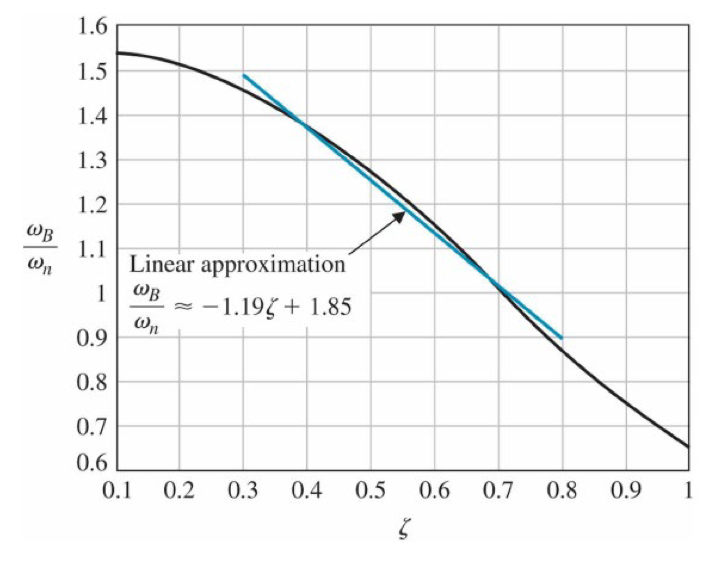
\includegraphics[width=0.5\linewidth]{./figures/bandwidth.png}
  \caption{Bandwidth against damping ratio.}
  \label{fig:bandwidth}
\end{figure}
So instead of bandwidth being equal to the natural frequency we have that:
\begin{equation*}
  \omega_B \approx \text{constant depending on } \xi \cdot \omega_n
.\end{equation*}
On \Cref{fig:bandwidth} we see that for $\xi = \num{0,5}$, $\omega_B / \omega_n \approx \num{1,27} $, so for $\xi = \num{0,5}$ we have that $\omega_B \approx \num{1,27}  \omega_n$.

\subsubsection{Relative Stability in the Frequency Domain}
We are now looking at the open-loop transfer function
\begin{equation*}
  L(j\omega) = G_c(j\omega) G(j\omega) H(j\omega)
\end{equation*}
and not the closed loop transfer function $T(j\omega)$.
E.g.
\begin{equation*}
  L(j\omega) = \frac{K}{j\omega \left( j\omega + 1 \right) \left( \num{0,2}j\omega + 2  \right)}
.\end{equation*}
The critical point for closed-loop stability is the point $-1 + j0$ in the complex $L(j\omega)$-plane.
On a Bode plot, that same point corresponds to $\left| L(j\omega) \right|= 1$, which is $20 \log \left| L(j\omega) \right| = \qty{0}{\dB} $ and phase $\angle L(j\omega) = \ang{-180}$.
So the dangerous situation is \qty{0}{\dB} and \ang{-180}.
I.e. if the open-loop system reaches magnitude 1 while having \ang{-180} phase, then the negative feedback effectively becomes positive feedback, which is why this point is critical.

On \Cref{fig:phasegainmarg} two important margins are shown.
First is the phase margin, i.e. how far the phase is from \ang{-180} at the frequency corresponding to a magnitude of \qty{0}{\dB} and the gain margin i.e. how far the magnitude is from \qty{0}{\dB} when the phase is \ang{-180}.
These margins tell us not just whether the system is stable, but how safely stable it is.

\begin{figure} [ht]
  \centering
  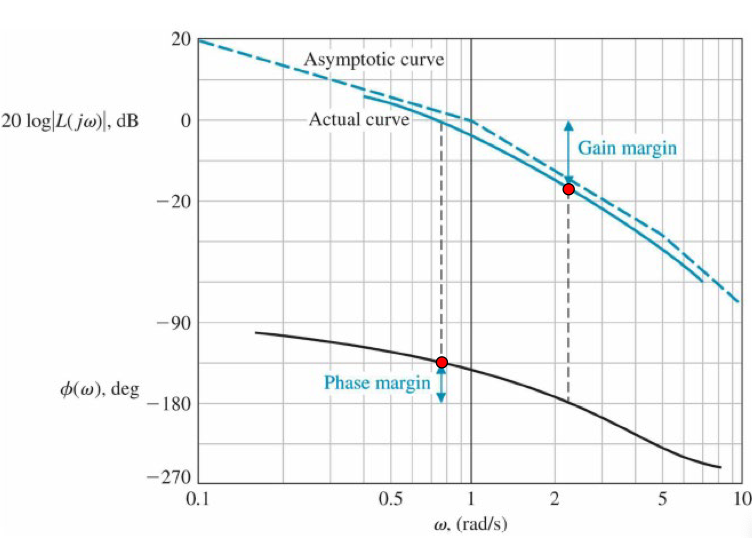
\includegraphics[width=0.5\linewidth]{./figures/phasegainmarg.png}
  \caption{Phase and gain margin.}
  \label{fig:phasegainmarg}
\end{figure}

The same margins idea can be applied to a log-magnitude-phase diagram (essentially a Nichols-style plot).
Instead of plotting magnitude and phase separately against frequency, we plot
\begin{equation*}
  20 \log \left| L(j\omega) \right|
\end{equation*}
against $\angle L(j\omega)$.
So the horizontal axis is the phase, and the vertical axis is magnitude in \unit{\dB}.
The critical points become very easy to see at \ang{-180} and \qty{0}{\dB}.
This is all shown on \Cref{fig:nichols}.

\begin{figure} [ht]
  \centering
  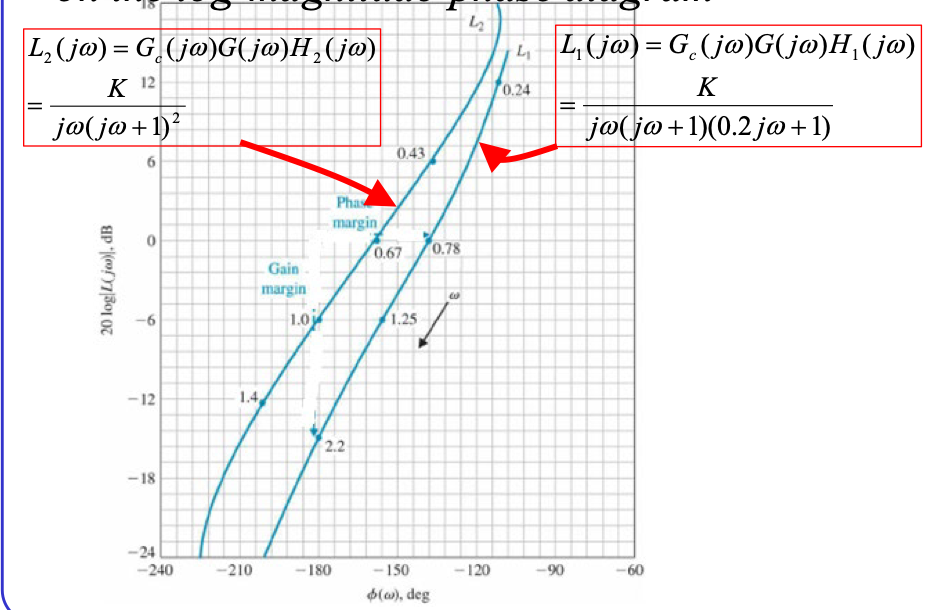
\includegraphics[width=0.5\linewidth]{./figures/nichols.png}
  \caption{Phase and gain margin on a log-magnitude-phase diagram.}
  \label{fig:nichols}
\end{figure}

The two curves on \Cref{fig:nichols} correspond to two loop transfer functions:
\begin{equation*}
  L_1(j\omega) = \frac{K}{j\omega \left( j\omega + 1 \right)\left( \num{0,2} j\omega + 1 \right)}
\end{equation*}
and
\begin{equation*}
  L_2(j\omega) = \frac{K}{j\omega \left( j\omega + 1 \right)^2}
.\end{equation*}
The closer the curve passes to the point $\left( \ang{-180}, \qty{0}{\dB} \right)$, the less stable the system is.

On \Cref{fig:nichols} the actual margins are, for $L_1$:
\begin{align*}
  \text{GM} &= \qty{15}{\dB}  \\
  \text{PM} &= \ang{43} 
\end{align*}
and for $L_2$:
\begin{align*}
  \text{GM} &= \qty{5,7}{\dB}  \\
  \text{PM} &= \ang{20} 
.\end{align*}
So $L_2$ is less stable than $L_1$ as its margins are smaller.
It can tolerate less extra gain and less extra phase lag before becoming unstable.

\paragraph{Phase Margins and Damping Ratios}
We now consider a second-order open-loop transfer function:
\begin{equation*}
  L(j\omega) = \frac{\omega_n^2}{s \left( s + 2\xi \omega_n \right)}
.\end{equation*}
This open-loop form gives a standard second-order closed-loop system.

The exact relationship between phase margin and damping ratio is shown on \Cref{fig:phasemargdamp} and given by:
\begin{equation*}
  \phi_{\text{pm}} = \tan^{-1} \frac{2}{\sqrt{\sqrt{4 + \frac{1}{\xi^{4}} -2}}}
.\end{equation*}
However an important approximation is $\xi = \num{0,01} \phi_{\text{pm}}$ for $\xi \leq \num{0,7} $, where $\phi_{\text{pm}}$ is measured in degrees.
So roughly:
\begin{align*}
  \text{PM} &= \ang{30} & \implies & \xi &\approx \num{0,3}  \\
  \text{PM} &= \ang{45}  & \implies & \xi &\approx \num{0,45}  \\
  \text{PM} &= \ang{60} & \implies & \xi &\approx \num{0,6} 
.\end{align*}

\begin{figure} [ht]
  \centering
  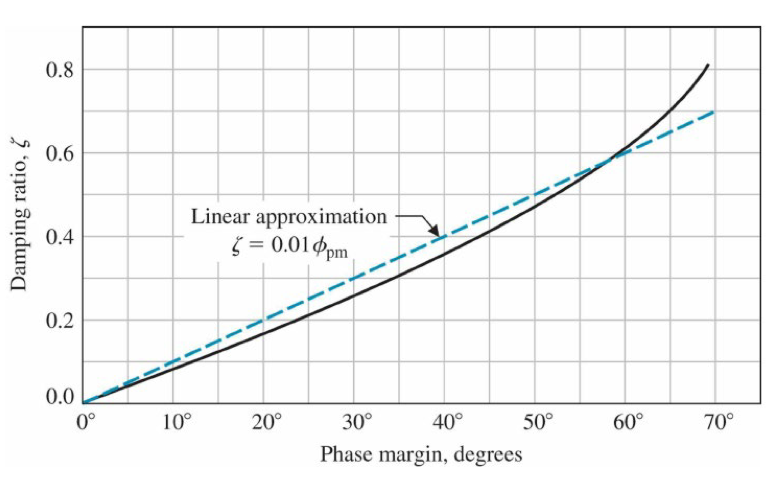
\includegraphics[width=0.5\linewidth]{./figures/phasemargdamp.png}
  \caption{Dependence of phase margins on damping ratio.}
  \label{fig:phasemargdamp}
\end{figure}

This is useful because damping ratio tells us about transient behavior.
A low damping ratio means more oscillation and overshoot and vice versa.

So phase-margins becomes a frequency-domain way of estimating transient response quality.

\paragraph{Margins versus gain $K$}
To show how stability margins change as the loop gain $K$ changes we use the example
\begin{equation*}
  L(s) = G_c(s) G(s) H(s) = \frac{K}{s \left( s + 4 \right)^2}
.\end{equation*}
As $K$ increases, the magnitude plot moves upwards.

That usually causes the gain crossover frequency to move to the right, where the system often has more phase lag, therefore, increasing $K$ tends to reduce the phase margin.
This is shown on the plots on \Cref{fig:phasemargk}.
Here we see the gain margin versus the gain $K$, the phase margin versus the gain $K$ and the gain margin versus the phase margin.

\begin{figure} [ht]
  \centering
  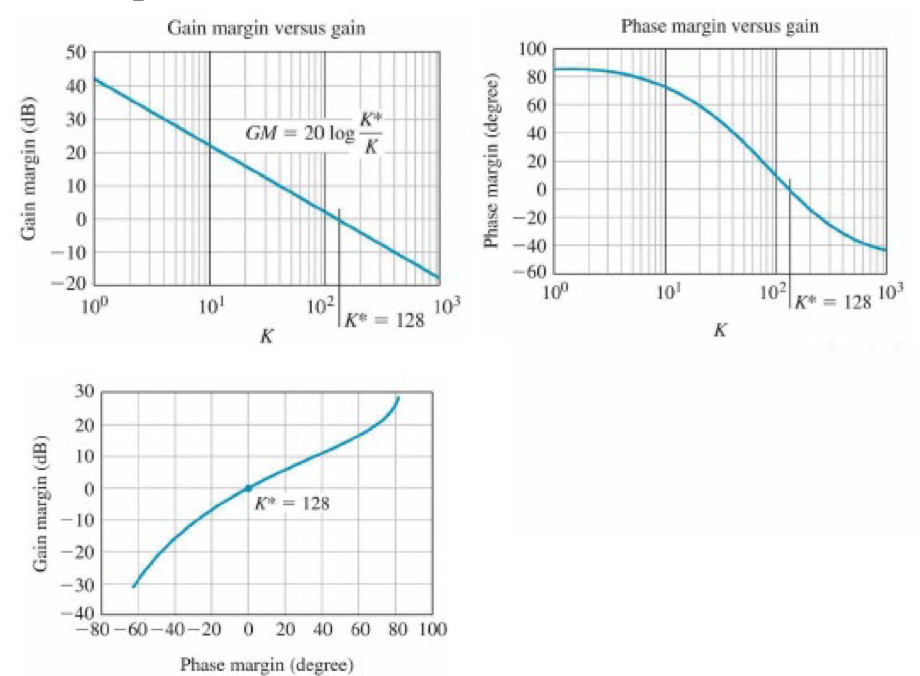
\includegraphics[width=0.5\linewidth]{./figures/phasemargk.png}
  \caption{Influence of gain $K$ on stability margins.}
  \label{fig:phasemargk}
\end{figure}

On \Cref{fig:phasemargk}, there is a critical value:
\begin{equation*}
  K^{*} = 128
.\end{equation*}
At this value, the system is marginally stable.
The gain margin is then \qty{0}{\dB} and the phase margin is approximately \ang{0}. 
Here:
\begin{equation*}
  \text{GM} = 20 \log \left( \frac{K^{*}}{K} \right)
.\end{equation*}
So if the current gain $K$ is much smaller than $K^{*}$ you have a large gain margin and vice versa.

\paragraph{Desired Frequency-Domain Specifications}
A good control system should have:
\begin{enumerate}
  \item Small resonant magnitude. E.g. $M_{p\omega} < \num{1,5}$, as a small resonant peak means less overshoot and better damping.
  \item Large bandwidth.
    A larger bandwidth usually means a faster time response, as this leads to transients dying out more quickly.
  \item A large phase margin.
    This helps keep the system away from the dangerous \ang{-180}, \qty{0}{\dB} point, meaning the system is less likely to become unstable.
\end{enumerate}

\subsubsection{Stability with Time Delays}
Now, we introduce time delays.
A time delay is the time between an action and its effect being observed somewhere in the system.

A pure time delay is represented by:
\begin{equation*}
  G_d(s) = e^{-sT}
\end{equation*}
where $T$ is the delay time.
Substituting $s = j\omega$, we get
\begin{equation*}
  G_d(j\omega) = e^{-j\omega T}
.\end{equation*}
The magnitude is:
\begin{equation*}
  \left| e^{-j\omega T} \right| = 1
\end{equation*}
so time delay does not change the magnitude plot.

But the phase is:
\begin{equation*}
  \phi(\omega) = -\omega T
\end{equation*}
in radians, and
\begin{equation*}
  \phi(\omega) = -\omega T \frac{\ang{180} }{\pi}
\end{equation*}
in degrees.
So time delay is dangerous because it adds phase lag without changing the magnitude.
On the Bode magnitude plot, nothing obvious happens, but on the phase plot, the system gets closer to \ang{-180}, so the phase margin decreases.
